\section{Problem}
There are several sub-problems in this system that the project needs to address. Here we present the main points affecting the architecture of the system together with our proposed solutions so far.
\subsection{Can system logic live outside of the server?}
This problem deals with how to avoid having crucial system logic and data on the server. If any server participating in the protocol goes down, will the system still be functional, given that another similar server is used instead?
\subsection{How can users verify the identities of their peers?}
Each user of the system will be associated with a self-generated private-public pair of cryptographic RSA keys. With knowledge of the public keys of their peers, there are standardized identity verification protocols used on a session-to-session basis. There is, however, a chicken-and-egg problem with the distribution of these public keys and how to tie them to identities. Traditionally, there are two types of Public Key Infrastructures (PKIs) with different ways to address this:
\begin{itemize}
\item A Web of Trust, as often utilized in OpenPGP. Here, a user has a list of peers that they trust - trusted introducers. If they receive a public key and associated identity signed by one of their trusted introducers, they will know that the trusted introducer has verified the connection between the identity and the public key. This way, an active user will steadily grow their network of trusted introducers. One needs to have a network of dependable and active peers in order to successfully participate in a Web of Trust.
\item A PKI centered around one or several Certificate Authorities (CAs). Here, there is a predefined list of authorities that are trusted to sign participants public keys. This creates a centralized network and puts a lot of trust in the CAs. SSL utilizes this approach and there are several historical examples of when this trust has been broken (more recently in the Diginotar hack of 2011).
\end{itemize}
For a truly decentralized system, it is not acceptable to adapt a CA-entered approach. While a Web of Trust is interesting, it might be too cumbersome for users. This issue is addressed in “Zooko’s Triangle” (See figure \ref{fig:zooko}), stating that no system assigning names to participants in a network can have the property that names are secure, decentralized and meaningful at the same time. This conjecture has since been proven false by the design of systems such as the blockchain of the cryptocurrency Namecoin, which effectively acts as a cryptographically secured distrubuted hash table (DHT) with unique keys. Namecoin is currently considered as a candidate for storing public keys with identities as keys. Perhaps a Web of Trust could be implemented on top of or beside this system.
\begin{figure}[h]
\centering
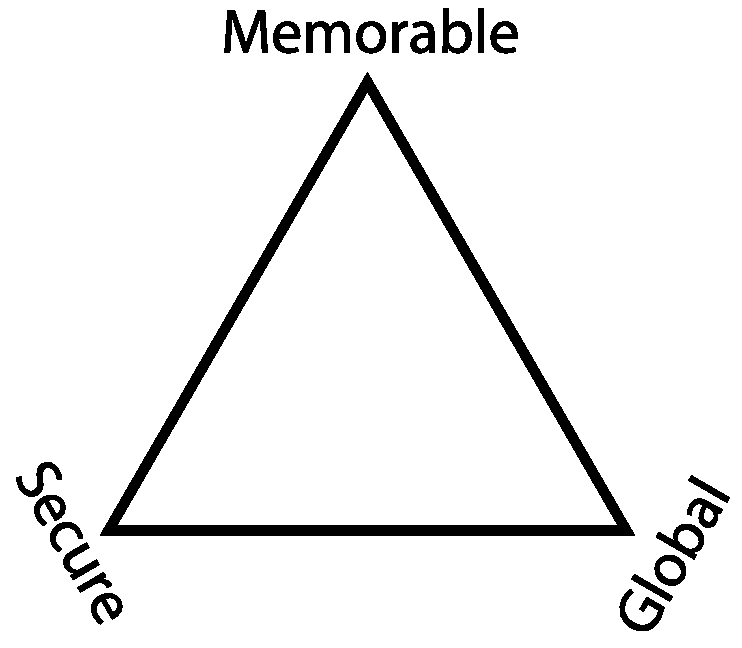
\includegraphics[width=\textwidth,height=0.2\paperheight,keepaspectratio
]{figures/Zooko_s_Triangle}
\caption{Zooko's Triangle, with the edges representing the achievable combinations of features \cite{Zooko:2001:Online}}
\label{fig:zooko}
\end{figure}

\subsection {How are resources stored?}
Usability, security and adherence to public web standards are three priorities that make the question of how to locally store resources on clients a difficult one. There are proprietary technologies for mapping resources to files on the local filesystem, which could be very useful – but without cross-platform support, it is considered out of the question for Rymd. Instead, it seems likely that resources will be stored in a local key-value store type database, where each resource is symmetrically encrypted with a corresponding secret key.

\subsection{How are resources identified?}
It is desirable for resources to have identifiers that are both memorable, secure, and unique - Zooko’s triangle is a concern here as well. However, there are practical limitations on using any current cryptocurrency blockchain here – the practical issues involved in creating and updating entries would make such a system practically unusable. Therefore, the most reasonable option seems to be for clients to assign randomly generated Globally Unique Identifiers (GUIDs) to each of their own resources. File names are not even close to unique and disclose unnecessary information, should an adversary without the corresponding secret key get hold of an encrypted resource. Since resources are communicated peer-to-peer, the issue of malicious GUID collision attacks becomes negligible since users would have first-hand contact with peers that they trust. Resource checksums will have to be communicated and verified by peers before accepting a transfer

\subsection{How to store and distribute cryptographic keys?}
Assuming that the system can utilize a DHT such as a cryptocurrency blockchain for storage of the public part of RSA key pairs, the issue of how to interface a web application with the blockchain in a way that allows for verification of identities without putting too much trust in the HTTP/Namecoin gateway also needs to be addressed. Also, the initial insertion of the key requires monetary resources, and is perhaps something that should be solved outside of Rymd.
While the public key can be stored in a DHT, private keys need to be stored securely on each client, preferably without giving client code any direct access to the raw keys. How the initial generation of keys are performed also needs consideration. Finally, a secure way to store the encryption keys for encrypted resources needs to be addressed. The question of how these resource-associated secret keys are distributed is deemed an implementation-specific question and will be out of scope for the library, but handled in the prototype.

\subsection{How are transfers initiated?}
Once peers have verified each other’s identities, the question of how two peers start the transfer of a shared resource arises. This is also an implementation detail in the application using the library, but the general idea for the prototype looks like this, with the premise that Alice wants to share R with Bob (The names of participants and their identities are used interchangeably. It builds on the notion that there is a one-to-one mapping between users and identities and that all participants have a pre-determined understanding of this mapping):

\begin{enumerate}
  \item Alice and Bob add each others as friends in their clients.
  \item Alice gets Bob’s public key from the DHT.
  \item Bob get Alice’s public key from the DHT. 
  \item Alice and Bob submit their friend lists to the peer-to-peer-server, which sets up a direct connection between them.
  \item Alice tells Bob’s client that she wants to share something with him.
  \item They authenticate using each other’s public keys.
  \item Alice sends K, the secret key used to encrypt R, to Bob, and ID, the GUID of the resource associated with the key.
  \item Bob’s client stores K in its keychain.
 \item Bob can now request R from Alice. Bob requests R from Alice.
 \item Alice sends R to Bob.
\end{enumerate}

An alternative flow could look like this (1-4 as above):
\begin{enumerate}
\setcounter{enumi}{4}
\item Bob somehow gets hold of ID outside of the system. Maybe from a web page, or Alice has sent it in a private message.
\item Bob asks Alice for K.
\item Alice approves Bob’s request and sends him K.
\item Bob’s client stores K in its keychain.
\item Bob requests R from Alice.
\item Alice sends R to Bob.
\end{enumerate}
Using this alternative flow, an interesting RetroShare-style file sharing network could be implemented where Alice does not even need to have access to R. If she doesn’t, she can ask her other peers for it, who can ask their peers, until perhaps someone down the line has the resource asked for and can send it directly to Bob, with or without K. The library should allow for implementations like this, but it is considered out of scope for this prototype.
\subsection{Trust issues}
Since the system logic is completely client side, how can one trust the fact that the client code is not altered between executions? This issue is one of the reasons why a large part of the online community is considering client-side JavaScript encryption to be a generally bad practice. The code will be open for anybody to read, which must be a reality to keep in mind during the project. Security through obscurity is not a good practice, but will not be an option anyway.

\subsection{Choice of technologies}
The technologies involved will need to be evaluated with issues regarding stability, security and compatibility in mind. Even though Rymd will not work on all web browsers and types of environments there are, one still has to consider browser compatability and the future development of the technologies used. This work will include research with regards to how actively maintained a technology or tool is, and how well documented it is. 
























